\chapter{Design and Implementation}
\label{chapter:design}

In this chapter we introduce the design and implementation details of the
optimization techniques implemented in our proxy solution. The design is based on the requirements identified in the previous chapter.

We get started by discussing the overall design.

\section{Overall Design}

The proposed design in this thesis includes a proxy pair.

\begin{figure}[h]
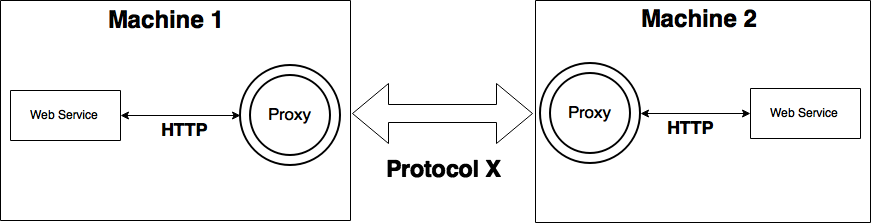
\includegraphics[scale=0.4]{images/architecture.png}
\caption{Architectural overview of proposed design}
\end{figure}


"By placing the first proxy as close to the client
as possible, preferably on the same physical
machine/device, challenges associated with TCP
and disadvantaged grids are avoided. This
deployment scheme ensures store-and-forward
capabilities throughout the network. Likewise,
for the last communications hop, between the
last proxy in the chain and the Web service,
standard HTTP and TCP is used, allowing inter-
operability with existing Web services without
requiring any modifications. By simply modifying
the URLs used by clients to invoke Web ser-
vices, the communication is routed through the
overlay network. Any instructions to the proxies
are specified as extra parameters added to the
URL. Apart from the modified URL, both Web
services clients and services are unaware of the
presence of the DSProxy system."

\section{Apache Camel}

This does the work of converting the specific input/request (like an HTTP
request) into something generic - a Camel Exchange - that can travel down a
Route.
 - quoute. må skrives om.


\section{DIL Proxy}

\subsection{Configuration}


\subsection{Routes and processors}

\subsection{Proxy header}

\subsection{Proxy setup}

In order to enable the applications to tunnel all their HTTP traffic through our
proxy, we needed a way to setup a proxy without altering the applications
themselves. Fortunately, Java provide mechanisms to deal with
proxies\cite{oracle-proxy}. We configured the \gls{jvm} to get the applications
to tunnel all HTTP traffic through our proxy. This is done by setting properties
to the \gls{jvm}:


\begin{lstlisting}[frame=single, caption="Setting a proxy on the \gls{jvm}", label=test]
java -Dhttp.proxyHost=localhost \
-Dhttp.proxyPort=3001 \
-Dhttp.nonProxyHosts= \
-jar target/client.jar
\end{lstlisting}

In \cref{test} the application \textbf{client.jar} is started and all HTTP
traffic will go through the proxy server at localhost on port 3001.


\section{Summary}
